\documentclass[aspectratio=169,11pt]{beamer}
\usetheme[progressbar=frametitle,numbering=fraction,sectionpage=none]{metropolis}
\usepackage{graphicx,booktabs,amsmath,amssymb,array}
\usepackage{tikz}
\usetikzlibrary{arrows.meta,positioning,shapes.geometric,calc}
\usepackage{pgfplots}
\pgfplotsset{compat=1.18}
\usepackage{fontawesome5}
\graphicspath{{../figs/}}

\definecolor{triad}{HTML}{D9541E}
\definecolor{simple}{HTML}{2A7AB0}
\definecolor{neural}{HTML}{8C8C8C}
\definecolor{neural2}{HTML}{BDBDBD}
\definecolor{soft}{HTML}{F3F1EC}
\setbeamercolor{alerted text}{fg=triad}

\title{TRIAD: Bundle Completion from Shared Relations}
\subtitle{Instead of learning every item, learn how items go together}
\author{Ajit and Soumen}
\date{}

\begin{document}
\maketitle

% =====================================================================================================================
\section{Motivation}

\begin{frame}{Bundles are everywhere}
\centering
\begin{columns}[T]
\column{.31\textwidth}\centering
{\Huge\color{triad}\faTshirt}\\[6pt]
\textbf{Outfits}\\[2pt]
\small top + trousers + shoes
\column{.31\textwidth}\centering
{\Huge\color{triad}\faMusic}\\[6pt]
\textbf{Playlists}\\[2pt]
\small songs around a few artists
\column{.31\textwidth}\centering
{\Huge\color{triad}\faShoppingCart}\\[6pt]
\textbf{Product kits}\\[2pt]
\small laptop + bag + mouse
\end{columns}
\vfill
\begin{block}{}
\centering Platforms rarely build bundles from nothing.\\
A stylist picks one or two items \alert{and the system suggests the rest}.
\end{block}
\end{frame}

\begin{frame}{Why it is hard: bundle data are long-tailed}
\begin{columns}[c]
\column{.5\textwidth}
\begin{itemize}
\item Catalogues: \textbf{3.5\,k to 254\,k} items
\item Training bundles: \textbf{1.2\,k to 21\,k}
\item Most items appear in a \alert{handful} of bundles
\item Many test targets appear in \alert{none}
\end{itemize}
\column{.5\textwidth}
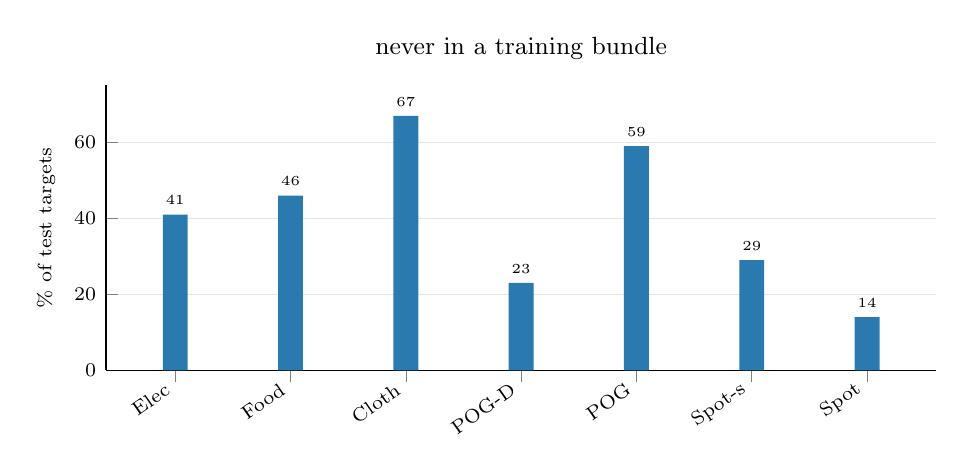
\begin{tikzpicture}
\begin{axis}[ybar, area legend, width=\linewidth, height=5.2cm, bar width=9pt, ymin=0, ymax=75,
  symbolic x coords={Elec,Food,Cloth,POG-D,POG,Spot-s,Spot}, xtick=data,
  x tick label style={rotate=35,anchor=east,font=\scriptsize}, y tick label style={font=\scriptsize},
  ylabel={\scriptsize \% of test targets}, title={\small never in a training bundle},
  nodes near coords, nodes near coords style={font=\tiny}, axis lines*=left, ymajorgrids, grid style={gray!20}]
\addplot[fill=simple, draw=none] coordinates {(Elec,41) (Food,46) (Cloth,67) (POG-D,23) (POG,59) (Spot-s,29) (Spot,14)};
\end{axis}
\end{tikzpicture}
\end{columns}
\end{frame}

% =====================================================================================================================
\section{Problem statement}

\begin{frame}{Bundle completion}
\centering
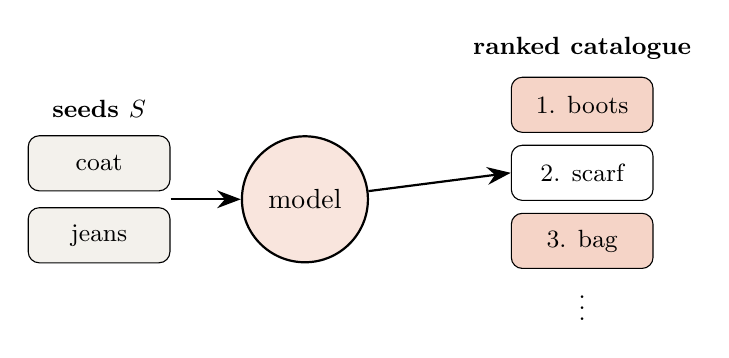
\begin{tikzpicture}[node distance=6mm, item/.style={draw, rounded corners, minimum width=18mm, minimum height=7mm, font=\small},
  arr/.style={-{Stealth[length=3mm]}, thick}]
\node[item, fill=soft] (s1) {coat};
\node[item, fill=soft, below=2mm of s1] (s2) {jeans};
\node[above=1mm of s1, font=\small\bfseries] {seeds $S$};
\node[draw, thick, circle, minimum size=16mm, right=18mm of $(s1)!.5!(s2)$, fill=triad!15] (m) {model};
\draw[arr] ($(s1.east)!.5!(s2.east)$) -- (m);
\node[item, right=18mm of m, yshift=12mm, fill=triad!25] (r1) {1. boots};
\node[item, below=1.5mm of r1] (r2) {2. scarf};
\node[item, below=1.5mm of r2, fill=triad!25] (r3) {3. bag};
\node[below=0mm of r3, font=\small] {$\vdots$};
\node[above=1mm of r1, font=\small\bfseries] {ranked catalogue};
\draw[arr] (m) -- ($(r1.west)!.5!(r3.west)$);
\end{tikzpicture}
\vfill
\begin{columns}[T]
\column{.48\textwidth}
\textbf{Input}: a few items of a bundle (the \emph{seeds})\\
\textbf{Output}: the whole catalogue, ranked
\column{.48\textwidth}
\textbf{Goal}: the missing items come first\\
\textbf{Metric}: Recall@20, NDCG@20, full catalogue
\end{columns}
\end{frame}

\begin{frame}{What makes it different from recommendation}
\begin{itemize}
\item The query is a \alert{set of items}, not a user
\item The answer must fit the seeds \alert{as a group}
\item Learned from \alert{existing bundles} made by experts, users or crowd workers
\end{itemize}
\vfill
\centering
\begin{tabular}{lll}
\toprule
Domain & Bundles made by & Datasets\\
\midrule
Fashion & Taobao fashion experts & POG, POG\_DENSE\\
Music & Spotify users & Spotify, Spotify\_sparse\\
E-commerce & crowd workers (Amazon sessions) & Electronic, Food, Clothing\\
\bottomrule
\end{tabular}
\end{frame}

% =====================================================================================================================
\section{Existing methods}

\begin{frame}{Recent models learn a vector for every item}
\centering
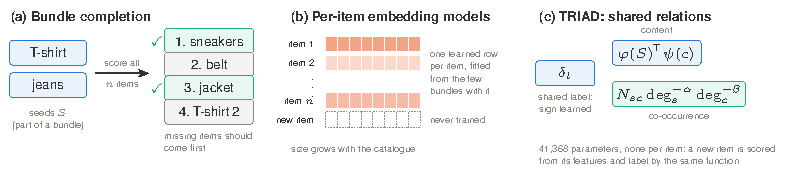
\includegraphics[width=.95\textwidth]{fig1.pdf}\\[4pt]
{\small (b) per-item models store knowledge in one learned row per item}
\end{frame}

% [hidden for now: DDBC / Bundle-MLLM] \begin{frame}{Four recent models, growing in size}
\begin{frame}{Recent models, growing in size}
\centering\small
\begin{tabular}{llr}
\toprule
Model & Idea & Size\\
\midrule
CLHE \small(WSDM'24) & multimodal + graph item views, self-attention & 3.7\,M -- 29\,M\\
RaMen \small(ECAI'25) & adds item--item graph and hypergraph & 1.3\,M -- 67\,M\\
% [hidden for now: DDBC / Bundle-MLLM] Bundle-MLLM \small(KDD'25) & fine-tuned Llama-2, 1 of 10 candidates & 7\,B\\
% [hidden for now: DDBC / Bundle-MLLM] DDBC \small(ICLR'26) & discrete diffusion over item codes & per-item codes\\

\bottomrule
\end{tabular}
\vfill
\begin{alertblock}{Two things in common}
\begin{itemize}
\item Each item gets its own learned representation
\item \textbf{None} is compared with co-occurrence or neighbourhood methods
\end{itemize}
\end{alertblock}
\end{frame}

% =====================================================================================================================
\section{Simple baselines beat neural models}

\begin{frame}{Tuned simple methods match or beat CLHE and RaMen}
\centering
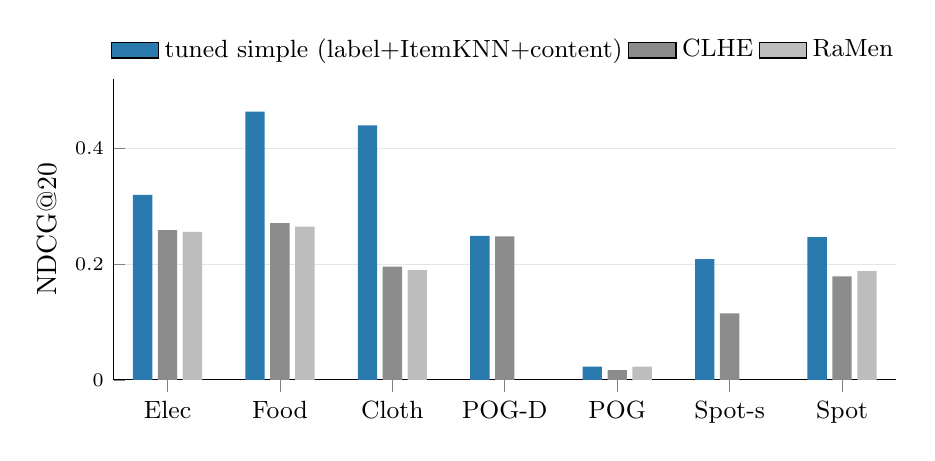
\begin{tikzpicture}
\begin{axis}[ybar, area legend, width=.95\textwidth, height=5.4cm, bar width=7pt, ymin=0, ymax=.52,
  symbolic x coords={Elec,Food,Cloth,POG-D,POG,Spot-s,Spot}, xtick=data,
  x tick label style={font=\small}, y tick label style={font=\scriptsize}, ylabel={NDCG@20},
  legend style={at={(.5,1.02)}, anchor=south, legend columns=3, font=\small, draw=none},
  axis lines*=left, ymajorgrids, grid style={gray!20}, enlarge x limits=.08]
\addplot[fill=simple, draw=none] coordinates {(Elec,.320) (Food,.464) (Cloth,.440) (POG-D,.249) (POG,.023) (Spot-s,.209) (Spot,.247)};
\addplot[fill=neural, draw=none] coordinates {(Elec,.259) (Food,.271) (Cloth,.196) (POG-D,.248) (POG,.017) (Spot-s,.115) (Spot,.179)};
\addplot[fill=neural2, draw=none] coordinates {(Elec,.256) (Food,.265) (Cloth,.190) (POG,.023) (Spot,.188)};
\legend{tuned simple (label+ItemKNN+content), CLHE, RaMen}
\end{axis}
\end{tikzpicture}\\
{\scriptsize Same splits, same features, three seeds. RaMen on POG and Spotify: published numbers. CLHE on Spotify: one seed.}
\end{frame}

% [hidden for now: DDBC / Bundle-MLLM] \begin{frame}{Also under the other papers' own protocols}
% [hidden for now: DDBC / Bundle-MLLM] \begin{columns}[T]
% [hidden for now: DDBC / Bundle-MLLM] \column{.5\textwidth}\centering
% [hidden for now: DDBC / Bundle-MLLM] \textbf{DDBC's protocol} (F1)\\[2pt]
% [hidden for now: DDBC / Bundle-MLLM] \begin{tikzpicture}
% [hidden for now: DDBC / Bundle-MLLM] \begin{axis}[ybar, area legend, width=\linewidth, height=5.2cm, bar width=7pt, ymin=0, ymax=.7,
% [hidden for now: DDBC / Bundle-MLLM]   symbolic x coords={POG-D,Spot-30,Spot-60,Spot-90}, xtick=data, x tick label style={font=\scriptsize},
% [hidden for now: DDBC / Bundle-MLLM]   y tick label style={font=\scriptsize}, legend style={at={(.5,1.02)},anchor=south,legend columns=2,font=\scriptsize,draw=none},
% [hidden for now: DDBC / Bundle-MLLM]   axis lines*=left, ymajorgrids, grid style={gray!20}, enlarge x limits=.15]
% [hidden for now: DDBC / Bundle-MLLM] \addplot[fill=simple, draw=none] coordinates {(POG-D,.452) (Spot-30,.544) (Spot-60,.562) (Spot-90,.564)};
% [hidden for now: DDBC / Bundle-MLLM] \addplot[fill=neural, draw=none] coordinates {(POG-D,.138) (Spot-30,.279) (Spot-60,.285) (Spot-90,.278)};
% [hidden for now: DDBC / Bundle-MLLM] \legend{simple, DDBC (rerun)}
% [hidden for now: DDBC / Bundle-MLLM] \end{axis}
% [hidden for now: DDBC / Bundle-MLLM] \end{tikzpicture}\\
% [hidden for now: DDBC / Bundle-MLLM] {\small simple $\approx$ \alert{2--3$\times$} DDBC}
% [hidden for now: DDBC / Bundle-MLLM] \column{.5\textwidth}\centering
% [hidden for now: DDBC / Bundle-MLLM] \textbf{Bundle-MLLM's protocol} (HitRate@1)\\[2pt]
% [hidden for now: DDBC / Bundle-MLLM] \begin{tikzpicture}
% [hidden for now: DDBC / Bundle-MLLM] \begin{axis}[ybar, area legend, width=\linewidth, height=5.2cm, bar width=7pt, ymin=0, ymax=1,
% [hidden for now: DDBC / Bundle-MLLM]   symbolic x coords={POG-D,POG,Spot-s,Spot}, xtick=data, x tick label style={font=\scriptsize},
% [hidden for now: DDBC / Bundle-MLLM]   y tick label style={font=\scriptsize}, legend style={at={(.5,1.02)},anchor=south,legend columns=2,font=\scriptsize,draw=none},
% [hidden for now: DDBC / Bundle-MLLM]   axis lines*=left, ymajorgrids, grid style={gray!20}, enlarge x limits=.15]
% [hidden for now: DDBC / Bundle-MLLM] \addplot[fill=simple, draw=none] coordinates {(POG-D,.617) (POG,.306) (Spot-s,.641) (Spot,.759)};
% [hidden for now: DDBC / Bundle-MLLM] \addplot[fill=neural, draw=none] coordinates {(POG-D,.668) (POG,.413) (Spot-s,.796) (Spot,.824)};
% [hidden for now: DDBC / Bundle-MLLM] \legend{simple, Bundle-MLLM (published)}
% [hidden for now: DDBC / Bundle-MLLM] \end{axis}
% [hidden for now: DDBC / Bundle-MLLM] \end{tikzpicture}\\
% [hidden for now: DDBC / Bundle-MLLM] {\small the one exception: simple falls \alert{below}}
% [hidden for now: DDBC / Bundle-MLLM] \end{columns}
% [hidden for now: DDBC / Bundle-MLLM] \end{frame}

\begin{frame}[standout]
Simple methods were never tested\\[4pt]
% [hidden for now: DDBC / Bundle-MLLM] and they beat 3 of the 4 recent models
and they match or beat both CLHE and RaMen
\end{frame}

% =====================================================================================================================
\section{Our method: TRIAD}

\begin{frame}{The idea: learn how items go together, not what each item is}
\begin{columns}[T]
\column{.32\textwidth}\centering
{\Huge\color{triad}\faEye}\\[4pt]
\textbf{Content}\\
\small does it look like it belongs?
\column{.32\textwidth}\centering
{\Huge\color{triad}\faTags}\\[4pt]
\textbf{Labels}\\
\small does it share a category or artist, and is that good?
\column{.32\textwidth}\centering
{\Huge\color{triad}\faProjectDiagram}\\[4pt]
\textbf{Co-occurrence}\\
\small has it been bundled with the seeds?
\end{columns}
\vfill
\begin{block}{}
\centering A \textbf{gate} decides, per query, how much to trust each answer.\\
Seeds seen in many bundles: trust counts. \quad Unseen seeds: trust content and labels.
\end{block}
\end{frame}

\begin{frame}{Inputs: three sources, computed once}
\centering
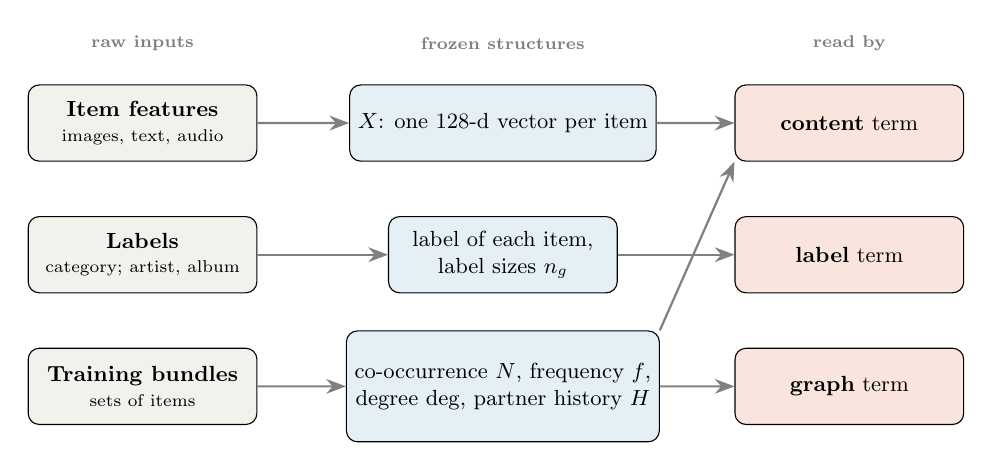
\begin{tikzpicture}[scale=.88, transform shape, font=\small, box/.style={draw, rounded corners, align=center, minimum width=33mm, minimum height=11mm},
  arr/.style={-{Stealth[length=2.5mm]}, thick, gray}]
\node[box, fill=soft] (f) at (0,1.9) {\textbf{Item features}\\[-1pt]\scriptsize images, text, audio};
\node[box, fill=soft] (l) at (0,0) {\textbf{Labels}\\[-1pt]\scriptsize category; artist, album};
\node[box, fill=soft] (b) at (0,-1.9) {\textbf{Training bundles}\\[-1pt]\scriptsize sets of items};
\node[box, fill=simple!12] (x) at (5.2,1.9) {$X$: one 128-d vector per item};
\node[box, fill=simple!12] (g) at (5.2,0) {label of each item,\\ label sizes $n_g$};
\node[box, fill=simple!12, minimum height=16mm] (n) at (5.2,-1.9) {co-occurrence $N$, frequency $f$,\\ degree $\deg$, partner history $H$};
\node[box, fill=triad!15] (c) at (10.2,1.9) {\textbf{content} term};
\node[box, fill=triad!15] (lt) at (10.2,0) {\textbf{label} term};
\node[box, fill=triad!15] (gr) at (10.2,-1.9) {\textbf{graph} term};
\draw[arr] (f) -- (x); \draw[arr] (l) -- (g); \draw[arr] (b) -- (n);
\draw[arr] (x) -- (c); \draw[arr] (g) -- (lt); \draw[arr] (n) -- (gr); \draw[arr] (n.north east) -- (c.south west);
\node[font=\scriptsize\bfseries, gray] at (0,3.05) {raw inputs};
\node[font=\scriptsize\bfseries, gray] at (5.2,3.05) {frozen structures};
\node[font=\scriptsize\bfseries, gray] at (10.2,3.05) {read by};
\end{tikzpicture}\\[6pt]
{\small Per query: the \alert{seeds $S$}. Nothing above is trained; only how the terms use it.}
\end{frame}

\begin{frame}{Item features: one 128-d vector per item}
\centering\small
\setlength{\tabcolsep}{4pt}
\begin{tabular}{lll}
\toprule
Datasets & Modality 1 & Modality 2\\
\midrule
POG, POG\_DENSE & BLIP image (768-d) & BLIP text of description (768-d)\\
Spotify, Spotify\_sparse & CLAP audio (512-d) & CLAP text of metadata (512-d)\\
Electronic, Food, Clothing & BLIP text of the title (768-d) & none\\
\bottomrule
\end{tabular}
\vfill
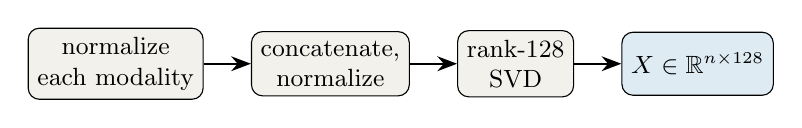
\begin{tikzpicture}[font=\small, stp/.style={draw, rounded corners, fill=soft, minimum height=8mm, align=center},
  arr/.style={-{Stealth[length=2.5mm]}, thick}]
\node[stp] (a) {normalize\\each modality};
\node[stp, right=6mm of a] (b) {concatenate,\\normalize};
\node[stp, right=6mm of b] (c) {rank-128\\SVD};
\node[stp, right=6mm of c, fill=simple!15] (d) {$X\in\mathbb{R}^{n\times128}$};
\draw[arr] (a)--(b); \draw[arr] (b)--(c); \draw[arr] (c)--(d);
\end{tikzpicture}
\vfill
{\small No bundle and no label is used. The simple content baselines get \alert{the same $X$}.}
\end{frame}

\begin{frame}{Architecture}
\centering
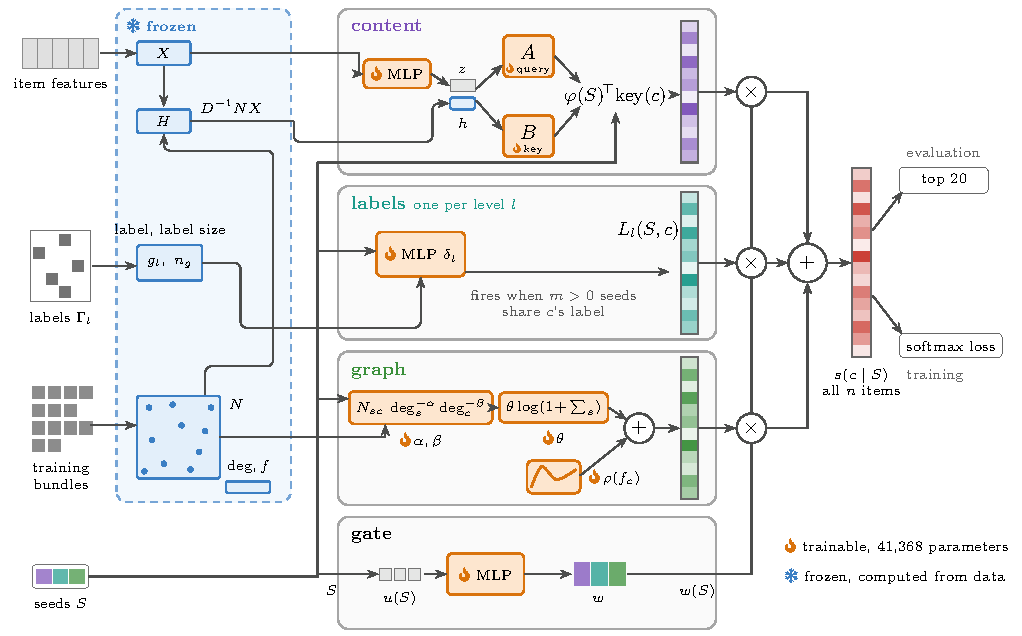
\includegraphics[height=.76\textheight]{fig2_arch.pdf}\\
{\small 41,368 trained parameters, \alert{none} belongs to an item}
\end{frame}









\begin{frame}{The score}
\[
s(c\mid S)=w_C(S)\,\underbrace{C(S,c)}_{\text{content}}+\textstyle\sum_l w_l(S)\,\underbrace{L_l(S,c)}_{\text{labels}}+w_G(S)\,\underbrace{G(S,c)}_{\text{graph}}
\]
\begin{columns}[T]
\column{.48\textwidth}\small
\begin{itemize}
\item three answers for every candidate $c$
\item weights $w(S)$ from the \alert{gate}, one per term
\item all $n$ items scored at once, ranked
\end{itemize}
\column{.5\textwidth}
\begin{block}{Real query (Electronic)}
\small seeds: two \textbf{DVD drives}\quad missing: a \textbf{hard drive}\\[3pt]
$s=1.54\times6.66+0.19\times0+4.60\times1.70=\mathbf{18.05}$\\[2pt]
highest of 3,497 items: \alert{ranked 1st}
\end{block}
\end{columns}
\end{frame}

\begin{frame}{Content: what the bundle needs vs.\ what the item offers}
\begin{columns}[c]
\column{.55\textwidth}\centering
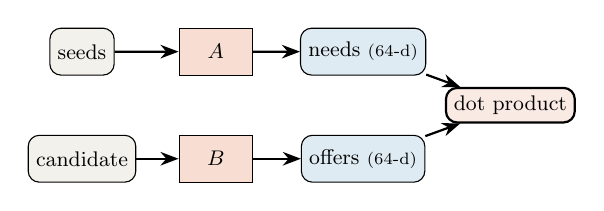
\begin{tikzpicture}[scale=.85, transform shape, font=\small, v/.style={draw, rounded corners, fill=soft, minimum height=7mm, align=center},
  m/.style={draw, fill=triad!20, minimum width=11mm, minimum height=7mm}, arr/.style={-{Stealth[length=2.3mm]}, thick}]
\node[v] (s) at (0,1) {seeds};
\node[m] (a) at (2,1) {$A$};
\node[v, fill=simple!15] (q) at (4.2,1) {needs \scriptsize(64-d)};
\node[v] (c) at (0,-.6) {candidate};
\node[m] (b) at (2,-.6) {$B$};
\node[v, fill=simple!15] (k) at (4.2,-.6) {offers \scriptsize(64-d)};
\node[draw, thick, rounded corners, fill=triad!12] (sc) at (6.4,.2) {dot product};
\draw[arr] (s)--(a); \draw[arr] (a)--(q); \draw[arr] (c)--(b); \draw[arr] (b)--(k); \draw[arr] (q)--(sc); \draw[arr] (k)--(sc);
\end{tikzpicture}\\[4pt]
{\scriptsize input: item features and \emph{partner history}\\ (what the item was bundled with)}
\column{.42\textwidth}
\begin{itemize}\small
\item $A\neq B$: \alert{asymmetric}\\ a shirt needs trousers, not more shirts
\item starts as plain feature similarity
\end{itemize}
\vspace{2mm}
\begin{block}{Example}\small
hard drive: $C=6.66$\\
other DVD drives: $C=7.20$\\
content alone would rank the target \textbf{37th}
\end{block}
\end{columns}
\end{frame}

\begin{frame}{Labels: is sharing a label good or bad?}
\begin{columns}[c]
\column{.55\textwidth}
\begin{itemize}
\item fires when the candidate \alert{shares a label} with a seed\\ (category; artist, album)
\item a small function of: how many seeds share it, query size, label size
\item its \alert{sign is learned}
\end{itemize}
\column{.42\textwidth}
\begin{block}{Learned}\small
outfits: shared category $\Rightarrow$ \textbf{$-$22.5}\\
playlists: shared artist $\Rightarrow$ \textbf{+1.88}\\[3pt]
example: another DVD drive $\Rightarrow$ +0.63\\
hard drive (no shared category) $\Rightarrow$ 0
\end{block}
\end{columns}
\end{frame}

\begin{frame}{Graph: has it been bundled with the seeds?}
\begin{columns}[c]
\column{.55\textwidth}
{\small\[
G=\theta\log\!\Big(1+\textstyle\sum_{s}N_{sc}\,\deg_s^{-\alpha}\deg_c^{-\beta}\Big)+\rho(f_c)
\]}
\begin{itemize}\small
\item co-occurrence counts, \alert{discounted} for items bundled with everything
\item discount powers $\alpha,\beta$ are \alert{learned}
\item a learned \alert{popularity prior} $\rho$
\end{itemize}
\column{.42\textwidth}
\begin{block}{Example}\small
hard drive bundled with the seeds 1 and 2 times\\[2pt]
$\Rightarrow G=1.70$\\[3pt]
never-bundled DVD drives: no counts, prior only
\end{block}
\end{columns}
\end{frame}

\begin{frame}{Gate: how much to trust each answer}
\begin{columns}[c]
\column{.55\textwidth}
Reads three numbers about the query:
\begin{enumerate}\small
\item how many seeds
\item how often the seeds were bundled
\item share of seeds never bundled
\end{enumerate}
\vspace{2mm}
\small Unseen seeds: no counts to rely on $\Rightarrow$ weight moves to \alert{content and labels}
\column{.42\textwidth}
\begin{block}{Example}\small
both seeds seen in training\\[2pt]
$w_C=1.54,\ w_{\text{label}}=0.19,\ w_G=\mathbf{4.60}$\\[2pt]
co-occurrence trusted \textbf{3$\times$} more than content
\end{block}
\end{columns}
\end{frame}

\begin{frame}{Training without leakage}
\begin{columns}[c]
\column{.55\textwidth}
\begin{itemize}
\item A training bundle sits inside the counts used to score it
\item The model would learn to \alert{read the answer} from its own counts
\item So each bundle is scored with \textbf{its own contribution removed}
\end{itemize}
\vspace{2mm}
{\small $N_{sc}-1$ for pairs inside the bundle, $\deg-(|b|-1)$, $f-1$}
\column{.42\textwidth}\centering
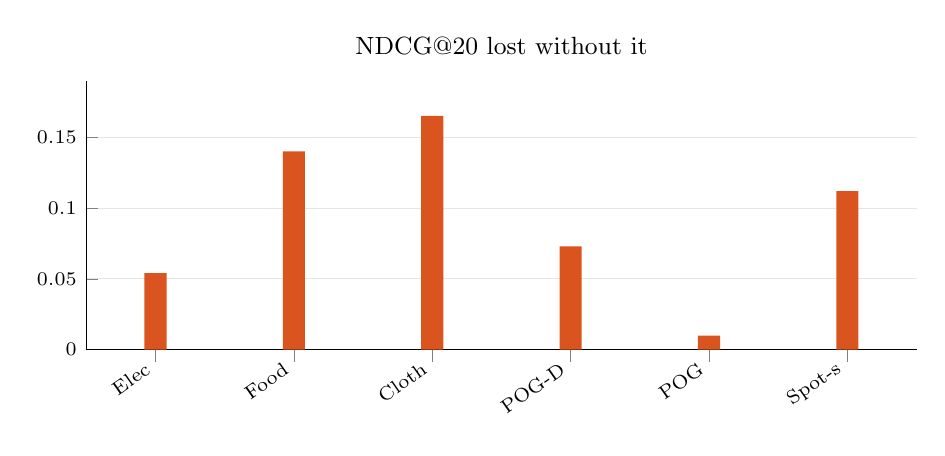
\begin{tikzpicture}
\begin{axis}[ybar, area legend, width=\linewidth, height=5cm, bar width=8pt, ymin=0, ymax=.19,
  symbolic x coords={Elec,Food,Cloth,POG-D,POG,Spot-s}, xtick=data, x tick label style={rotate=35,anchor=east,font=\scriptsize},
  y tick label style={font=\scriptsize,/pgf/number format/fixed}, scaled y ticks=false, title={\small NDCG@20 lost without it}, axis lines*=left, ymajorgrids, grid style={gray!20}]
\addplot[fill=triad, draw=none] coordinates {(Elec,.054) (Food,.140) (Cloth,.165) (POG-D,.073) (POG,.010) (Spot-s,.112)};
\end{axis}
\end{tikzpicture}
\end{columns}
\end{frame}

\begin{frame}{How it differs from a tuned blend}
\begin{columns}[T]
\column{.48\textwidth}
\textbf{Tuned blend}
\begin{itemize}\small
\item one fixed weight per dataset
\item discounts set by grid search
\item same-label rule fixed by hand
\item content = cosine similarity
\end{itemize}
\column{.48\textwidth}
\textbf{TRIAD}
\begin{itemize}\small
\item \alert{per-query} weights (gate)
\item discounts and prior \alert{learned jointly}
\item label rule's \alert{sign learned}
\item asymmetric content that scores \alert{complements}
\end{itemize}
\end{columns}
\vfill
\centering\small Ablations: gate up to \textbf{.065} NDCG@20, leave-one-out up to \textbf{.165}, training \textbf{.030--.179}
\end{frame}

% =====================================================================================================================
\section{Results}

\begin{frame}{TRIAD scores above every model}
\centering
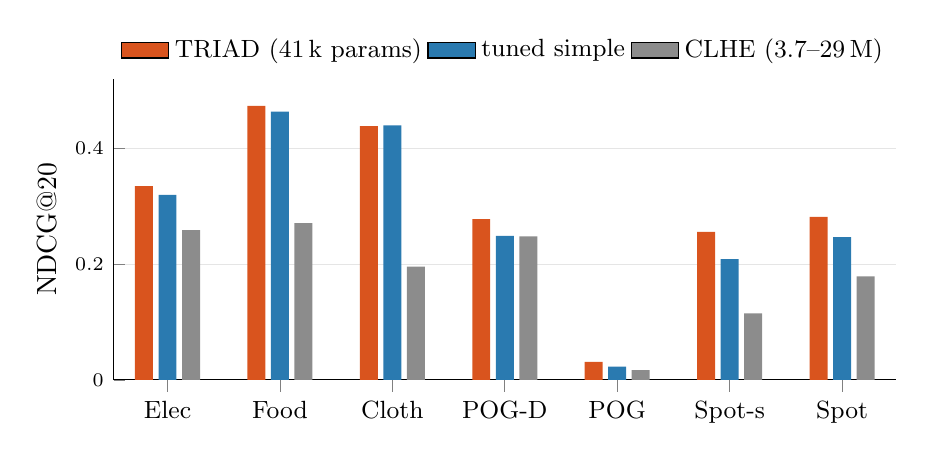
\begin{tikzpicture}
\begin{axis}[ybar, area legend, width=.95\textwidth, height=5.4cm, bar width=6.5pt, ymin=0, ymax=.52,
  symbolic x coords={Elec,Food,Cloth,POG-D,POG,Spot-s,Spot}, xtick=data,
  x tick label style={font=\small}, y tick label style={font=\scriptsize}, ylabel={NDCG@20},
  legend style={at={(.5,1.02)}, anchor=south, legend columns=3, font=\small, draw=none},
  axis lines*=left, ymajorgrids, grid style={gray!20}, enlarge x limits=.08]
\addplot[fill=triad, draw=none] coordinates {(Elec,.335) (Food,.474) (Cloth,.439) (POG-D,.278) (POG,.031) (Spot-s,.256) (Spot,.282)};
\addplot[fill=simple, draw=none] coordinates {(Elec,.320) (Food,.464) (Cloth,.440) (POG-D,.249) (POG,.023) (Spot-s,.209) (Spot,.247)};
\addplot[fill=neural, draw=none] coordinates {(Elec,.259) (Food,.271) (Cloth,.196) (POG-D,.248) (POG,.017) (Spot-s,.115) (Spot,.179)};
\legend{TRIAD (41\,k params), tuned simple, CLHE (3.7--29\,M)}
\end{axis}
\end{tikzpicture}\\
{\small Outfits and playlists: \alert{significantly ahead} of the best simple method. E-commerce: level.}
\end{frame}

\begin{frame}{A benchmark effect we isolate}
\begin{columns}[c]
\column{.55\textwidth}
\begin{itemize}
\item Catalogues hold \alert{only items that occur in some bundle}
\item So a never-bundled item is probably a test target
\item TRIAD learns this from training data alone
\item We give the baselines the same prior, and report TRIAD without it
\end{itemize}
\column{.42\textwidth}
\begin{block}{Add never-bundled items}
\begin{itemize}\small
\item the learned bonus shrinks, then turns into a penalty
\item its gain falls to \textbf{zero}
\item TRIAD stays level with simple
\end{itemize}
\end{block}
\end{columns}
\vfill
\centering\small On short e-commerce bundles most of the gain comes from this effect, for every method.
\end{frame}

\begin{frame}{TRIAD learns readable rules}
\begin{columns}[c]
\column{.52\textwidth}\centering
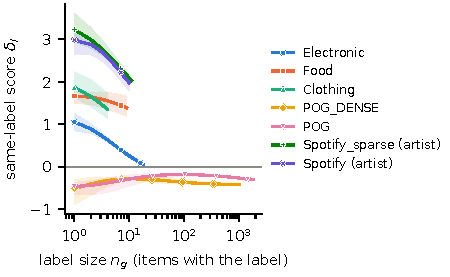
\includegraphics[width=\linewidth]{fig4_delta.pdf}
\column{.46\textwidth}
\begin{itemize}
\item Same function, \alert{sign learned per domain}
\item Outfits: a shared category is a \textbf{strong penalty} ($-$22.5)
\item Playlists: a shared artist is a \textbf{reward} (+1.88)
\item Nobody told the model either rule
\end{itemize}
\end{columns}
\end{frame}

\begin{frame}{How much data does it need?}
\centering
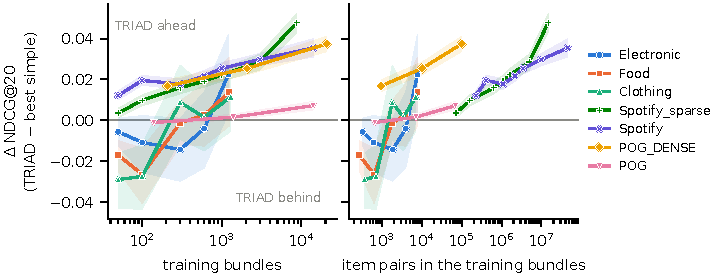
\includegraphics[width=.92\textwidth]{fig3_budget.pdf}\\[4pt]
\small Playlists: ahead down to \textbf{50} bundles. \quad E-commerce: behind with \textbf{100 or fewer}.
\end{frame}

% =====================================================================================================================
\section{Takeaways}

\begin{frame}{Takeaways}
\begin{enumerate}
% [hidden for now: DDBC / Bundle-MLLM] \item Bundle completion does \alert{not need a vector per item}: 41\,k shared parameters beat models of 1--67\,M and 7\,B
\item Bundle completion does \alert{not need a vector per item}: 41\,k shared parameters beat models of 1--67\,M
% [hidden for now: DDBC / Bundle-MLLM] \item Tuned \alert{simple methods} belong in every comparison: they beat 3 of 4 recent models
\item Tuned \alert{simple methods} belong in every comparison: they match or beat CLHE and RaMen
\item \alert{Benchmark construction} can look like modelling progress: control for it
\item Learning pays off where bundles carry structure (outfits, playlists), not yet on tiny e-commerce sets
\end{enumerate}
\end{frame}

\end{document}
